% ------------------------------------------------------------------------------
% TYPO3 Version 11.0 - What's New (English Version)
%
% @author	Michael Schams <schams.net>
% @license	Creative Commons BY-NC-SA 3.0
% @link		https://typo3.org/help/documentation/whats-new/
% @language	English
% ------------------------------------------------------------------------------

\documentclass[t]{beamer}

% suppress navigation bar
\beamertemplatenavigationsymbolsempty

\mode<presentation>
{
	\usetheme{typo3slides}
}

% global variables
\title{TYPO3 Version 11.0 - What's New}
\subtitle{Summary of the new features, changes and improvements}
\author{
	\centerline{Created by:}
	\centerline{Michael Schams}
}

\date{\today}

\begin{document}

% select TYPO3 Share font
\sharefont

% ------------------------------------------------------------------------------
% Title Page
% ------------------------------------------------------------------------------

\begingroup
	\setbeamercolor{normal text}{fg=white,bg=typo3orange}
	\setbeamercolor{title}{fg=white}
	\setbeamercolor{author}{fg=white}
	\setbeamertemplate{footline}[default]
	\begin{frame}
		\titlepage
	\end{frame}
\endgroup

% ------------------------------------------------------------------------------
% Table of Contents
% ------------------------------------------------------------------------------

\section*{TYPO3 Version 11.0 - What's New}
\begin{frame}[fragile]
	\frametitle{Chapter Overview}
	\framesubtitle{Chapter Overview}

	\tableofcontents

\end{frame}

% ------------------------------------------------------------------------------

% Chapter "Introduction"
% ------------------------------------------------------------------------------
% TYPO3 Version 11.0 - What's New (Dutch Version)
%
% @license	Creative Commons BY-NC-SA 3.0
% @link		http://typo3.org/download/release-notes/whats-new/
% @language	Dutch
% ------------------------------------------------------------------------------

\section{Wijzigingen voor integrators en ontwikkelaars}
\begin{frame}[fragile]
	\frametitle{Wijzigingen voor integrators en ontwikkelaars}

	\begin{center}\huge{Hoofdstuk 2:}\end{center}
	\begin{center}\huge{\color{typo3darkgrey}\textbf{Wijzigingen voor integrators en ontwikkelaars}}\end{center}

\end{frame}

% ------------------------------------------------------------------------------

% ------------------------------------------------------------------------------
% TYPO3 Version 11.0 - What's New (English Version)
%
% @author	Michael Schams <schams.net>
% @license	Creative Commons BY-NC-SA 3.0
% @link		https://typo3.org/help/documentation/whats-new/
% @language	English
% ------------------------------------------------------------------------------
% TYPO3 Version 11.0 - The Facts

\begin{frame}[fragile]
	\frametitle{Introduction}
	\framesubtitle{TYPO3 Version 11.0 - The Facts}

	\begin{itemize}
		\item Release date: 22 December 2020
		\item Release type: Sprint Release
	\end{itemize}

	\begin{figure}
		
\includegraphics[width=0.95\linewidth]{Introduction/typo3-v11-0-banner.png}
	\end{figure}

\end{frame}

% ------------------------------------------------------------------------------

% ------------------------------------------------------------------------------
% TYPO3 Version 11.0 - What's New (German Version)
%
% @license	Creative Commons BY-NC-SA 3.0
% @link		https://typo3.org/help/documentation/whats-new/
% @language	German
% ------------------------------------------------------------------------------
% TYPO3 Version 11.0 - Executive Summary

\begin{frame}[fragile]
	\frametitle{Einführung}
	\framesubtitle{Zusammenfassung}

	\small
		TYPO3 Version 11.0 ist das erste Sprint Release auf dem Weg zur LTS-Version
		(Long Term Support) im Jahr 2021.

		\vspace{0.2cm}

		Da der Schwerpunkt der Version 11.0 auf Aufräumarbeiten liegt, ist es nicht unerwartet,
		dass in dieser Version eine große Anzahl von wichtigen Änderungen eingeführt wurde.

		\vspace{0.2cm}

		Dieser Ansatz erlaubt es uns, neue Bibliotheken, moderne Konzepte und
		optimierte APIs in einem frühen Stadium der Entwicklung einzuführen, um sicherzustellen, dass TYPO3
		eines der besten Enterprise Content Management-Systeme auf dem Markt bleibt.

		\vspace{0.2cm}

%		Various exciting
%		\href{https://typo3.org/community/teams/typo3-development/initiatives/}{initiatives}
%		have also been formed to make long-term improvements in specific areas of
%		TYPO3.
	\normalsize

\end{frame}

% ------------------------------------------------------------------------------

% ------------------------------------------------------------------------------
% TYPO3 Version 11.0 - What's New (French Version)
%
% @license	Creative Commons BY-NC-SA 3.0
% @link		https://typo3.org/help/documentation/whats-new/
% @language	French
% ------------------------------------------------------------------------------
% System Requirements

\begin{frame}[fragile]
	\frametitle{Introduction}
	\framesubtitle{System Requirements}

	\begin{itemize}
		\item Version de PHP~: 7.4+
		\item Configuration PHP~:

			\begin{itemize}
				\item \texttt{memory\_limit} >= 256M
				\item \texttt{max\_execution\_time} >= 240s
				\item \texttt{max\_input\_vars} >= 1500
				\item L'option de compilation \texttt{-}\texttt{-disable-ipv6}
				\underline{NE} doit \underline{PAS} être utilisée
			\end{itemize}

		\item La majorité des serveurs de base de données supportés par \textbf{Doctrine DBAL}
			fonctionnent avec TYPO3. Les moteurs testés sont par exemple~:
	\end{itemize}

	\begin{figure}
		
\includegraphics[width=0.80\linewidth]{Introduction/logo-databases.png}
	\end{figure}

\end{frame}

% ------------------------------------------------------------------------------

% ------------------------------------------------------------------------------
% TYPO3 Version 11.0 - What's New (German Version)
%
% @license	Creative Commons BY-NC-SA 3.0
% @link		https://typo3.org/help/documentation/whats-new/
% @language	German
% ------------------------------------------------------------------------------
% Development, Support, and Maintenance Timeline

\begin{frame}[fragile]
	\frametitle{Einführung}
	\framesubtitle{Entwicklung, Support und Instandhaltung}

	\textbf{TYPO3 v11}

	\begin{figure}
		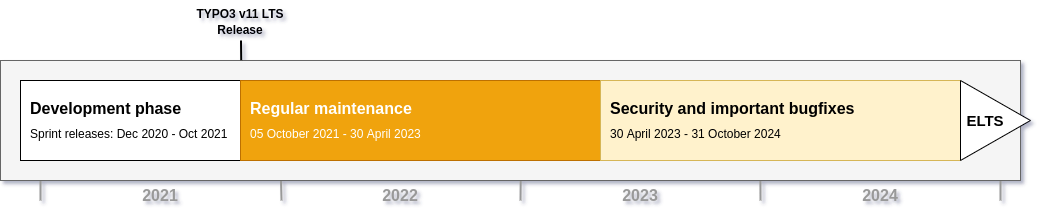
\includegraphics[width=1\linewidth]{Introduction/typo3-v11-lifecycle.png}
	\end{figure}

	\textbf{Erweiterte langfristige Unterstützung (ELTS)}\newline
	\smaller
		Die \href{https://typo3.com}{TYPO3 GmbH} bietet weitere Supportmöglichkeiten
		für TYPO3 v11 LTS auch nach dem 31. Oktober 2024 für bis zu zwei weitere Jahre.
	\normalsize

\end{frame}

% ------------------------------------------------------------------------------

% ------------------------------------------------------------------------------
% TYPO3 Version 11.0 - What's New (German Version)
%
% @license	Creative Commons BY-NC-SA 3.0
% @link		https://typo3.org/help/documentation/whats-new/
% @language	German
% ------------------------------------------------------------------------------
% TYPO3 v11 Release Dates

\begin{frame}[fragile]
	\frametitle{Einführung}
	\framesubtitle{TYPO3 v11 Roadmap}

	Voraussichtliche Veröffentlichungen und deren Hauptfokus:

	\begin{itemize}
		\item
			\begingroup
				\color{typo3orange}
				v11.0 \tabto{1.1cm}22/Dez/2020\tabto{3.4cm}New system requirements and breaking changes
			\endgroup
		\item v11.1 \tabto{1.1cm}23/Feb/2021\tabto{3.4cm}Multi-factor authentication
		\item v11.2 \tabto{1.1cm}04/Mai/2021\tabto{3.4cm}Link sharing for TYPO3 Backend
		\item v11.3 \tabto{1.1cm}13/Jul/2021\tabto{3.4cm}(\textit{to be determined})
		\item v11.4 \tabto{1.1cm}07/Sep/2021\tabto{3.4cm}Feature freeze
		\item v11.5 \tabto{1.1cm}05/Okt/2021\tabto{3.4cm}LTS Release (Long-term Support)

	\end{itemize}

	\smaller
		\url{https://typo3.org/cms/roadmap}\newline
		\url{https://typo3.org/article/a-first-glimpse-of-typo3-v11}
	\normalsize

\end{frame}

% ------------------------------------------------------------------------------

% ------------------------------------------------------------------------------
% TYPO3 Version 11.0 - What's New (Dutch Version)
%
% @license	Creative Commons BY-NC-SA 3.0
% @link		https://typo3.org/help/documentation/whats-new/
% @language	Dutch
% ------------------------------------------------------------------------------
% Installation

\begin{frame}[fragile]
	\frametitle{Introduction}
	\framesubtitle{Installation}

	% decrease font size for code listing
	\lstset{basicstyle=\fontsize{8}{10}\ttfamily}

	\begin{itemize}
		\item Official \textit{classic} installation procedure under Linux/Mac OS X\newline
			(DocumentRoot for example \texttt{/var/www/site/htdocs}):
\begin{lstlisting}
$ cd /var/www/site
$ wget --content-disposition get.typo3.org/11.0
$ tar xzf typo3_src-11.0.0.tar.gz
$ cd htdocs
$ ln -s ../typo3_src-11.0.0 typo3_src
$ ln -s typo3_src/index.php
$ ln -s typo3_src/typo3
$ touch FIRST_INSTALL
\end{lstlisting}

		\item See \href{https://docs.typo3.org/m/typo3/guide-installation/master/en-us/}{Installation and Upgrade Guide}
			for details about Microsoft Windows systems.

	\end{itemize}
\end{frame}

% ------------------------------------------------------------------------------

% ------------------------------------------------------------------------------
% TYPO3 Version 11.0 - What's New (English Version)
%
% @author	Michael Schams <schams.net>
% @license	Creative Commons BY-NC-SA 3.0
% @link		https://typo3.org/help/documentation/whats-new/
% @language	English
% ------------------------------------------------------------------------------
% Installation using Composer

\begin{frame}[fragile]
	\frametitle{Installation and Upgrade}
	\framesubtitle{Installation Using \texttt{Composer}}

	\begin{itemize}
		\item Installation using \textit{composer} under Linux, macOS, and Windows 10:
			\begin{lstlisting}
$ cd /var/www/site/
$ composer create-project typo3/cms-base-distribution typo3v11 ^11
			\end{lstlisting}

		\item Alternatively, create your custom \texttt{composer.json} file and run:
			\begin{lstlisting}
$ composer install
			\end{lstlisting}

			Further details are available in the
			\href{https://docs.typo3.org/m/typo3/guide-installation/master/en-us/}{Installation and Upgrade Guide}.

	\end{itemize}
\end{frame}

% ------------------------------------------------------------------------------


% Chapter "Backend User Interface"
% ------------------------------------------------------------------------------
% TYPO3 Version 11.0 - What's New (Dutch Version)
%
% @license	Creative Commons BY-NC-SA 3.0
% @link		http://typo3.org/download/release-notes/whats-new/
% @language	Dutch
% ------------------------------------------------------------------------------

\section{Wijzigingen voor integrators en ontwikkelaars}
\begin{frame}[fragile]
	\frametitle{Wijzigingen voor integrators en ontwikkelaars}

	\begin{center}\huge{Hoofdstuk 2:}\end{center}
	\begin{center}\huge{\color{typo3darkgrey}\textbf{Wijzigingen voor integrators en ontwikkelaars}}\end{center}

\end{frame}

% ------------------------------------------------------------------------------

% ------------------------------------------------------------------------------
% TYPO3 Version 11.0 - What's New (English Version)
%
% @author	Michael Schams <schams.net>
% @license	Creative Commons BY-NC-SA 3.0
% @link		http://typo3.org/download/release-notes/whats-new/
% @language	English
% ------------------------------------------------------------------------------

\begin{frame}[fragile]
	\frametitle{BackendUserInterface}
	\framesubtitle{Bootstrap Version 5}

	The TYPO3 backend now uses Bootstrap version 5.
	\newline
	...

\end{frame}

% ------------------------------------------------------------------------------

% ------------------------------------------------------------------------------
% TYPO3 Version 11.0 - What's New (English Version)
%
% @author	Michael Schams <schams.net>
% @license	Creative Commons BY-NC-SA 3.0
% @link		http://typo3.org/download/release-notes/whats-new/
% @language	English
% ------------------------------------------------------------------------------
% Breaking | 92582 | Resizable text area user setting dropped

\begin{frame}[fragile]
	\frametitle{Backend User Interface}
	\framesubtitle{Resizable Text Area}

	The user setting "\textbf{Make text areas flexible}" has been removed and is no longer available for backend users.
	Text areas now always resize to the maximum height.

	\begin{figure}
		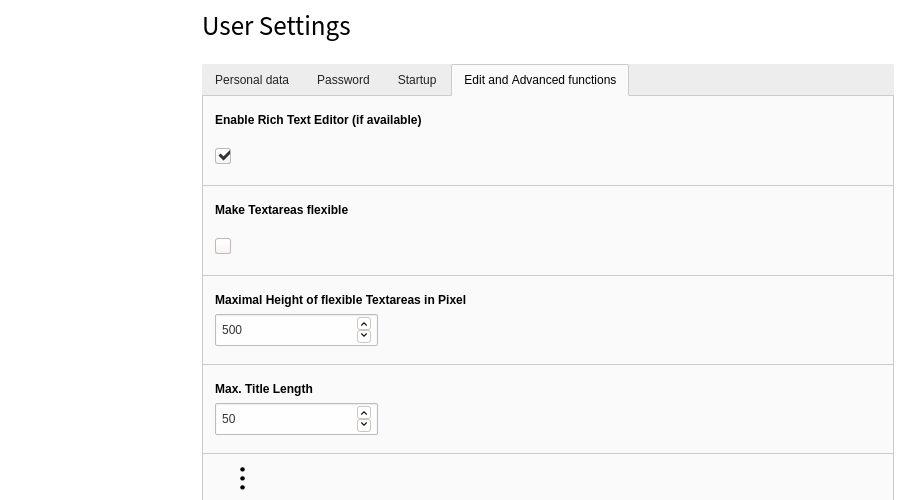
\includegraphics[width=1\linewidth]{BackendUserInterface/92582-ResizableTextArea.png}
	\end{figure}

\end{frame}

% ------------------------------------------------------------------------------


% Chapter "Changes for Integrators and Developers"
% ------------------------------------------------------------------------------
% TYPO3 Version 11.0 - What's New (Dutch Version)
%
% @license	Creative Commons BY-NC-SA 3.0
% @link		http://typo3.org/download/release-notes/whats-new/
% @language	Dutch
% ------------------------------------------------------------------------------

\section{Wijzigingen voor integrators en ontwikkelaars}
\begin{frame}[fragile]
	\frametitle{Wijzigingen voor integrators en ontwikkelaars}

	\begin{center}\huge{Hoofdstuk 2:}\end{center}
	\begin{center}\huge{\color{typo3darkgrey}\textbf{Wijzigingen voor integrators en ontwikkelaars}}\end{center}

\end{frame}

% ------------------------------------------------------------------------------

% ------------------------------------------------------------------------------
% TYPO3 Version 11.0 - What's New (English Version)
%
% @author	Michael Schams <schams.net>
% @license	Creative Commons BY-NC-SA 3.0
% @link		http://typo3.org/download/release-notes/whats-new/
% @language	English
% ------------------------------------------------------------------------------
% Deprecation | 92435 | Deprecated StandaloneView for EmailFinisher

\begin{frame}[fragile]
	\frametitle{Deprecated/Removed Functions}
	\framesubtitle{Form Framework}

	\begin{itemize}
		\item Since TYPO3 v10, integrators/developers can use Fluid-based emails
			in the \textit{EmailFinisher}. Therefore, the StandaloneView has now
			been marked as \textbf{deprecated}, along with the configuration
			option \texttt{templatePathAndFilename}.
		\item Item 2
		\item Item 3
	\end{itemize}

\end{frame}

% ------------------------------------------------------------------------------


% Chapter "Changes for Integrators"
% ------------------------------------------------------------------------------
% TYPO3 Version 11.0 - What's New (Dutch Version)
%
% @license	Creative Commons BY-NC-SA 3.0
% @link		http://typo3.org/download/release-notes/whats-new/
% @language	Dutch
% ------------------------------------------------------------------------------

\section{Wijzigingen voor integrators en ontwikkelaars}
\begin{frame}[fragile]
	\frametitle{Wijzigingen voor integrators en ontwikkelaars}

	\begin{center}\huge{Hoofdstuk 2:}\end{center}
	\begin{center}\huge{\color{typo3darkgrey}\textbf{Wijzigingen voor integrators en ontwikkelaars}}\end{center}

\end{frame}

% ------------------------------------------------------------------------------

% ------------------------------------------------------------------------------
% TYPO3 Version 11.0 - What's New (English Version)
%
% @author	Michael Schams <schams.net>
% @license	Creative Commons BY-NC-SA 3.0
% @link		http://typo3.org/download/release-notes/whats-new/
% @language	English
% ------------------------------------------------------------------------------

\begin{frame}[fragile]
	\frametitle{Changes for Integrators}
	\framesubtitle{Breaking Changes}

	\small
		Integrators be advised: In TYPO3 v10, some PHP code, TSconfig, TypoScript
		options and conditions, etc. were marked as deprecated.

		\vspace{0.2cm}

		In accordance to
		\href{https://typo3.org/article/typo3-deprecation-policy}{TYPO3's Deprecation Policy},
		these components have changed or were removed in TYPO3 v11.0.

		\vspace{0.2cm}

		Enable the deprecation log, carefully test your code, and review the log
		to locate possible issues. Use the built-in
		\href{https://docs.typo3.org/m/typo3/reference-coreapi/master/en-us/ApiOverview/ExtensionScanner/Index.html}{Extension Scanner}
		to get a full report of extension incompatibilities.

	\normalsize

\end{frame}

% ------------------------------------------------------------------------------

% ------------------------------------------------------------------------------
% TYPO3 Version 11.0 - What's New (English Version)
%
% @author	Michael Schams <schams.net>
% @license	Creative Commons BY-NC-SA 3.0
% @link		http://typo3.org/download/release-notes/whats-new/
% @language	English
% ------------------------------------------------------------------------------
% Breaking | 92457 | Extension Repository database table removed
% Feature | 92538 | Show extension constraints in extension manager
% Breaking | 92532 | Support for extension-in-extension installation in Extension Manager removed
% Breaking | 92590 | Removed support for extension upload of t3x files ★

\begin{frame}[fragile]
	\frametitle{Changes for Integrators}
	\framesubtitle{Extension Manager}

	\begin{itemize}

		\item The Extension Manager now features an \textit{all versions} view
			that shows detailed information about extensions.

		\item The following database table is not used anymore and was removed:
			\begin{itemize}\small
				\item \texttt{tx\_extensionmanager\_domain\_model\_repository}
			\end{itemize}\normalsize
			\vspace{0.2cm}

		\item The (undocumented) support for extension-in-extension installations
			has been removed. The following directory is now ignored:
			\begin{itemize}\small
				\item \texttt{EXT:my\_extension/Initialisation/Extensions/}
			\end{itemize}
			\vspace{0.2cm}

		\item As we have phased out the proprietary format \texttt{.t3x} in favor
			of \texttt{.zip} files, the feature of uploading \texttt{.t3x} files
			has been removed.

	\end{itemize}

\end{frame}

% ------------------------------------------------------------------------------

% ------------------------------------------------------------------------------
% TYPO3 Version 11.0 - What's New (English Version)
%
% @author	Michael Schams <schams.net>
% @license	Creative Commons BY-NC-SA 3.0
% @link		http://typo3.org/download/release-notes/whats-new/
% @language	English
% ------------------------------------------------------------------------------
% Important | 92870 | Always use Fluid based page module

\begin{frame}[fragile]
	\frametitle{Changes for Integrators}
	\framesubtitle{Feature Toggles}

	\begin{itemize}
		\item As TYPO3 now always uses the Fluid-based page module, the feature
			toggle to switch between different implementations has been removed.
		\item Item 2
		\item Item 3
	\end{itemize}

\end{frame}

% ------------------------------------------------------------------------------

% ------------------------------------------------------------------------------
% TYPO3 Version 11.0 - What's New (English Version)
%
% @author	Michael Schams <schams.net>
% @license	Creative Commons BY-NC-SA 3.0
% @link		http://typo3.org/download/release-notes/whats-new/
% @language	English
% ------------------------------------------------------------------------------
% Breaking | 92582 | Resizable text area user setting dropped

\begin{frame}[fragile]
	\frametitle{Backend User Interface}
	\framesubtitle{Resizable Text Area}

	The user setting "\textbf{Make text areas flexible}" has been removed and is no longer available for backend users.
	Text areas now always resize to the maximum height.

	\begin{figure}
		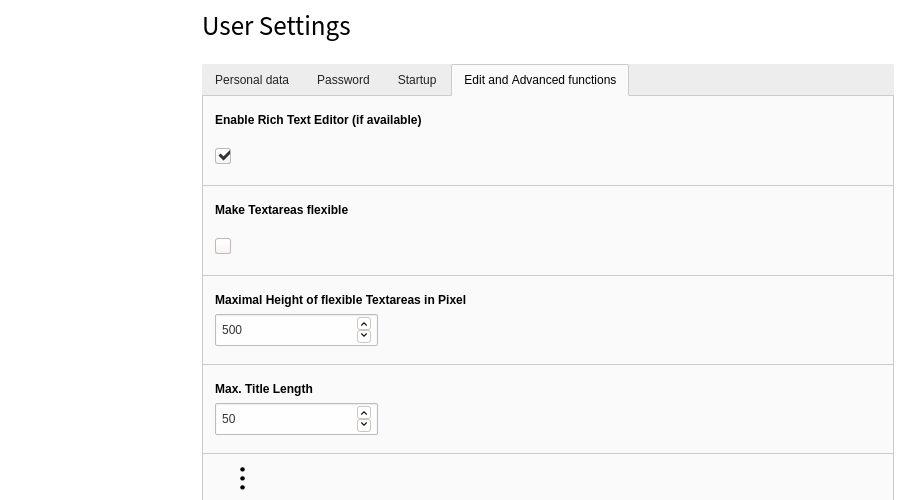
\includegraphics[width=1\linewidth]{BackendUserInterface/92582-ResizableTextArea.png}
	\end{figure}

\end{frame}

% ------------------------------------------------------------------------------

% ------------------------------------------------------------------------------
% TYPO3 Version 11.0 - What's New (English Version)
%
% @author	Michael Schams <schams.net>
% @license	Creative Commons BY-NC-SA 3.0
% @link		http://typo3.org/download/release-notes/whats-new/
% @language	English
% ------------------------------------------------------------------------------


% Chapter "Changes for Developers"
% ------------------------------------------------------------------------------
% TYPO3 Version 11.0 - What's New (Dutch Version)
%
% @license	Creative Commons BY-NC-SA 3.0
% @link		http://typo3.org/download/release-notes/whats-new/
% @language	Dutch
% ------------------------------------------------------------------------------

\section{Wijzigingen voor integrators en ontwikkelaars}
\begin{frame}[fragile]
	\frametitle{Wijzigingen voor integrators en ontwikkelaars}

	\begin{center}\huge{Hoofdstuk 2:}\end{center}
	\begin{center}\huge{\color{typo3darkgrey}\textbf{Wijzigingen voor integrators en ontwikkelaars}}\end{center}

\end{frame}

% ------------------------------------------------------------------------------

% ------------------------------------------------------------------------------
% TYPO3 Version 11.0 - What's New (English Version)
%
% @author	Michael Schams <schams.net>
% @license	Creative Commons BY-NC-SA 3.0
% @link		http://typo3.org/download/release-notes/whats-new/
% @language	English
% ------------------------------------------------------------------------------

\begin{frame}[fragile]
	\frametitle{Changes for Integrators}
	\framesubtitle{Breaking Changes}

	\small
		Integrators be advised: In TYPO3 v10, some PHP code, TSconfig, TypoScript
		options and conditions, etc. were marked as deprecated.

		\vspace{0.2cm}

		In accordance to
		\href{https://typo3.org/article/typo3-deprecation-policy}{TYPO3's Deprecation Policy},
		these components have changed or were removed in TYPO3 v11.0.

		\vspace{0.2cm}

		Enable the deprecation log, carefully test your code, and review the log
		to locate possible issues. Use the built-in
		\href{https://docs.typo3.org/m/typo3/reference-coreapi/master/en-us/ApiOverview/ExtensionScanner/Index.html}{Extension Scanner}
		to get a full report of extension incompatibilities.

	\normalsize

\end{frame}

% ------------------------------------------------------------------------------

% ------------------------------------------------------------------------------
% TYPO3 Version 11.0 - What's New (English Version)
%
% @author	Michael Schams <schams.net>
% @license	Creative Commons BY-NC-SA 3.0
% @link		http://typo3.org/download/release-notes/whats-new/
% @language	English
% ------------------------------------------------------------------------------
% Important | 92736 | Return timestamp as integer in DateTimeAspect

\begin{frame}[fragile]
	\frametitle{Changes for Developers}
	\framesubtitle{DateTimeAspect}

	\begin{itemize}
		\item The \texttt{DateTimeAspect} returns the timestamp as an integer now.
\begin{lstlisting}
$ context = GeneralUtility::makeInstance(Context::class);
$ timestamp = $context->getPropertyFromAspect('date', 'timestamp');
\end{lstlisting}

		\item Item 2
		\item Item 3
	\end{itemize}

\end{frame}

% ------------------------------------------------------------------------------

% ------------------------------------------------------------------------------
% TYPO3 Version 11.0 - What's New (English Version)
%
% @author	Michael Schams <schams.net>
% @license	Creative Commons BY-NC-SA 3.0
% @link		http://typo3.org/download/release-notes/whats-new/
% @language	English
% ------------------------------------------------------------------------------
% Breaking | 92502 | Make Extbase handle PSR-7 responses only

\begin{frame}[fragile]
	\frametitle{Changes for Developers}
	\framesubtitle{Extbase: PSR-7 Responses}

	\begin{itemize}
		\item Extbase now creates a
			\href{https://www.php-fig.org/psr/psr-7/}{PSR-7}-compatible
			response object and passes it back through the request handling stack.
		\item The following interfaces/classes are not used anymore and were removed:

			\begin{itemize}\small
				\item \texttt{TYPO3\textbackslash
					CMS\textbackslash
					Extbase\textbackslash
					Mvc\textbackslash
					ResponseInterface}
				\item \texttt{TYPO3\textbackslash
					CMS\textbackslash
					Extbase\textbackslash
					Mvc\textbackslash
					Response}
			\end{itemize}

		\item If a controller action should return custom data instead of the
			default view, a PSR-7-compatible response object can be returned:
\begin{lstlisting}
public function listAction()
{
  // do your action stuff
  return new \TYPO3\CMS\Core\Http\HtmlResponse($this->view->render());
}
\end{lstlisting}
	\end{itemize}

\end{frame}

% ------------------------------------------------------------------------------

% ------------------------------------------------------------------------------
% TYPO3 Version 11.0 - What's New (French Version)
%
% @license	Creative Commons BY-NC-SA 3.0
% @link		http://typo3.org/download/release-notes/whats-new/
% @language	French
% ------------------------------------------------------------------------------
% Feature | 92531 | Improved Email Validation

\begin{frame}[fragile]
	\frametitle{Changes for Developers}
	\framesubtitle{Email Validation}

	% decrease font size for code listing
	\lstset{basicstyle=\tiny\ttfamily}

	\begin{itemize}
		\item Developers can use the following method to validate email addresses:
			\newline\smaller
				\texttt{TYPO3\textbackslash
					CMS\textbackslash
					Core\textbackslash
					Utility\textbackslash
					GeneralUtility::validEmail()}\normalsize

		\item Since TYPO3 v11.0, it is possible to configure the validators
			and to implement custom solutions.

		\item For example:
\begin{lstlisting}
$GLOBALS['TYPO3_CONF_VARS']['MAIL']['validators'] = [
  \Egulias\EmailValidator\Validation\RFCValidation::class,
  \Egulias\EmailValidator\Validation\DNSCheckValidation::class
];
\end{lstlisting}

		\item The following default validators are available:
			\begin{itemize}\smaller
				\item \texttt{\textbackslash
					Egulias\textbackslash
					EmailValidator\textbackslash
					Validation\textbackslash
					RFCValidation} (used by default)
				\item \texttt{\textbackslash
					Egulias\textbackslash
					EmailValidator\textbackslash
					Validation\textbackslash
					DNSCheckValidation}
				\item \texttt{\textbackslash
					Egulias\textbackslash
					EmailValidator\textbackslash
					Validation\textbackslash
					SpoofCheckValidation}
				\item \texttt{\textbackslash
					Egulias\textbackslash
					EmailValidator\textbackslash
					Validation\textbackslash
					NoRFCWarningsValidation}
			\end{itemize}
	\end{itemize}

\end{frame}

% ------------------------------------------------------------------------------


% Chapter "Deprecated and Removed Functions"
% ------------------------------------------------------------------------------
% TYPO3 Version 11.0 - What's New (Dutch Version)
%
% @license	Creative Commons BY-NC-SA 3.0
% @link		http://typo3.org/download/release-notes/whats-new/
% @language	Dutch
% ------------------------------------------------------------------------------

\section{Wijzigingen voor integrators en ontwikkelaars}
\begin{frame}[fragile]
	\frametitle{Wijzigingen voor integrators en ontwikkelaars}

	\begin{center}\huge{Hoofdstuk 2:}\end{center}
	\begin{center}\huge{\color{typo3darkgrey}\textbf{Wijzigingen voor integrators en ontwikkelaars}}\end{center}

\end{frame}

% ------------------------------------------------------------------------------

% ------------------------------------------------------------------------------
% TYPO3 Version 11.0 - What's New (English Version)
%
% @author	Michael Schams <schams.net>
% @license	Creative Commons BY-NC-SA 3.0
% @link		http://typo3.org/download/release-notes/whats-new/
% @language	English
% ------------------------------------------------------------------------------
% Breaking | 89137 | Database fields t3ver_tstamp and t3ver_count dropped
% Breaking | 92457 | Extension Repository database table removed

\begin{frame}[fragile]
	\frametitle{Deprecated/Removed Functions}
	\framesubtitle{Database-related Changes (1)}

	\begin{itemize}
		\item The following two database fields were removed from various tables:
			\begin{itemize}\smaller
				\item \texttt{t3ver\_tstamp}
				\item \texttt{t3ver\_count}
			\end{itemize}\normalsize
			\vspace{0.4cm}

		\item The following database table is not used anymore and was removed:
			\begin{itemize}\smaller
				\item \texttt{tx\_extensionmanager\_domain\_model\_repository}
			\end{itemize}\normalsize
			\vspace{0.4cm}

		\item Item 3
	\end{itemize}

\end{frame}

% ------------------------------------------------------------------------------


% Chapter "Miscellaneous"
% ------------------------------------------------------------------------------
% TYPO3 Version 11.0 - What's New (Dutch Version)
%
% @license	Creative Commons BY-NC-SA 3.0
% @link		http://typo3.org/download/release-notes/whats-new/
% @language	Dutch
% ------------------------------------------------------------------------------

\section{Wijzigingen voor integrators en ontwikkelaars}
\begin{frame}[fragile]
	\frametitle{Wijzigingen voor integrators en ontwikkelaars}

	\begin{center}\huge{Hoofdstuk 2:}\end{center}
	\begin{center}\huge{\color{typo3darkgrey}\textbf{Wijzigingen voor integrators en ontwikkelaars}}\end{center}

\end{frame}

% ------------------------------------------------------------------------------

% ------------------------------------------------------------------------------
% TYPO3 Version 11.0 - What's New (English Version)
%
% @author	Michael Schams <schams.net>
% @license	Creative Commons BY-NC-SA 3.0
% @link		http://typo3.org/download/release-notes/whats-new/
% @language	English
% ------------------------------------------------------------------------------


% Chapter "Sources and Authors"
% ------------------------------------------------------------------------------
% TYPO3 Version 11.0 - What's New (Dutch Version)
%
% @license	Creative Commons BY-NC-SA 3.0
% @link		http://typo3.org/download/release-notes/whats-new/
% @language	Dutch
% ------------------------------------------------------------------------------

\section{Wijzigingen voor integrators en ontwikkelaars}
\begin{frame}[fragile]
	\frametitle{Wijzigingen voor integrators en ontwikkelaars}

	\begin{center}\huge{Hoofdstuk 2:}\end{center}
	\begin{center}\huge{\color{typo3darkgrey}\textbf{Wijzigingen voor integrators en ontwikkelaars}}\end{center}

\end{frame}

% ------------------------------------------------------------------------------

% ------------------------------------------------------------------------------
% TYPO3 Version 11.0 - What's New (Italian Version)
%
% @license	Creative Commons BY-NC-SA 3.0
% @link		http://typo3.org/download/release-notes/whats-new/
% @language	Italian
% ------------------------------------------------------------------------------
% Sources

\begin{frame}[fragile]
	\frametitle{Sources and Authors}
	\framesubtitle{Sources}

	\textbf{TYPO3 News:}
		\begin{itemize}\smaller
			\item \url{https://typo3.org/project/news/}
		\end{itemize}

	\textbf{Release Infos:}
		\begin{itemize}\smaller
			\item \url{https://get.typo3.org/release-notes/11.x/TYPO3_CMS_11.0.0}
			\item \href{https://docs.typo3.org/c/typo3/cms-core/master/en-us/Changelog-11.html}{TYPO3 v11 ChangeLog}
			\item \texttt{typo3/sysext/core/Documentation/Changelog/11.0/*}
		\end{itemize}

	\textbf{TYPO3 Bug-/Issuetracker:}
		\begin{itemize}\smaller
			\item \url{https://forge.typo3.org/projects/typo3cms-core}
		\end{itemize}

	\textbf{TYPO3 and Fluid Git Repositories:}
		\begin{itemize}\smaller
			\item \url{https://git.typo3.org/Packages/TYPO3.CMS.git}
			\item \url{https://github.com/TYPO3/Fluid}
		\end{itemize}

\end{frame}

% ------------------------------------------------------------------------------

% ------------------------------------------------------------------------------
% TYPO3 Version 11.0 - What's New (French Version)
%
% @license	Creative Commons BY-NC-SA 3.0
% @link		http://typo3.org/download/release-notes/whats-new/
% @language	French
% ------------------------------------------------------------------------------
% The TYPO3 CMS What's New Team

\begin{frame}[fragile]
	\frametitle{Sources et Auteurs}

	\vspace{-0.6cm}

	\centerline{\textbf{Équipe TYPO3 CMS What's New~:}}

	\begin{center}
		\centerline{Paul Blondiaux, Pierrick Caillon, Andreas Fießer,}
		\centerline{Richard Haeser, Jigal van Hemert, Henrietta Kucsovan, Corina Miron,}
		\centerline{Sinisa Mitrovic, Michael Schams, and Roberto Torresani}
	\end{center}

	\vspace{0.6cm}

	\smaller\begin{center}\url{https://typo3.org/help/documentation/whats-new/}\end{center}\normalsize

	\vspace{1cm}

	\smaller\begin{center}Sous license Creative Commons BY-NC-SA 3.0\end{center}\normalsize
	\begin{figure}\vspace*{-0.4cm}
		
\includegraphics[width=1.4cm]{SourcesAndAuthors/CreativeCommons-BY-NC-SA.png}
	\end{figure}

\end{frame}

% ------------------------------------------------------------------------------


% ------------------------------------------------------------------------------
\end{document}
